\section{Password Protection}
\label{passwordprotection}
After showing that user passwords are more guessable when their personal information is available, we wonder how users could protect their passwords from such attacks by mitigating the unwanted correlation between passwords and personal information. It is commonly believed that there is trade-off between password usability and security. A secure password would usually be less because it is expected to be long and random. However, people are bothered to remember secure passwords since the usability of secure passwords is low. In this work we seek an easy way to make passwords more secure while maintain acceptable memorability.

\subsection{Distortion Function}
We realize that making users remember passwords that are totally irrelevant to them is infeasible because users have much difficulty remembering them. Although most users concern their password security, many of them would not sacrifice password usability for security. Therefore we introduce distortion function, which is a function on that is applied on user passwords. The distortion function can be chosen by users so it could be linear or non-linear. If properly chosed, the distortion function is able to map user passwords to more secure strings. Distortion functions can serve its purpose by either break password semantics or increase password entropy. Therefore, the user only needs to remember the original password and a simple function to create a much stronger password. 

We conducted a proof-of-concept study to show the effectiveness of distortion function on password security. In our study, we use 2 types of distortion functions. 

For the first type of distortion function, every password symbol is mapped to another symbol. The mapping function can be chosen by users. In our study, we choose "add1" and "addpi" as 2 such distortion functions. "add1" simply rolls the character to the next one. For example, "a" rolls to "b", "z" rolls to "a" and "1" rolls to "2". "addpi" is a non-linear function. It rolls characters by the position specified by $\pi$, which is $31415 \ldots$. It means the first character rolls 3 position and the second rolls 1 position, etc.

The second distortion function adds an extra symbol between any pair of symbols in passwords. The length of passwords become twice of the original password minus 1. We call this distortion function "gapx", in which "x" represents the extra symbol. For example, when $x = "a"$, Alice's password "alice816" will be "aalaiacaea8a1a6" after the distortion function. In our study, we choose "gap0", "gapa", and "gap!".

Note in both types of the distortion functions we do not alter special characters. The distortion functions we used are some of the simplest. However, simple does not mean ineffective. After applying the distortion functions on each of the password in 12306 dataset. We again calculate the Coverage to study the effect of distortion functions. The result is shown in Figure~\ref{f4}. In general, these simple distortion functions would greatly reduce the correlation between user passwords and personal information. We notice that distortion functions are also generating different results. For example, we found "add!" performs best (Coverage is 0 for all users so it cannot been found in Figure~\ref{f4})since users rarely have personal information that has special characters) Surprisingly, "addpi" as the only non-linear function, does not produce better result than linear functions. We believe it is because digits which Chinese users prefer to use are likely to cause a coincidence match for its low entropy. Therefore no matter how the digits are mapped, there could be coincidence matches. However, these coincidence matches tend to be short in length, which does not raise Coverage much high as we stress continuation in match when computing Coverage. To conclude, distortion functions mitigates the problem of vast usage of personal information in user passwords while users can still remember the passwords. What is more, distortion function is also cure for semantics-aware password cracking methods, for example, A method \cite{veras2014semantic} proposed by R. Veras leverages semantic patterns in passwords to crack other passwords. After applying a distortion function, the semantic pattern would no longer be available, thus make the passwords secure against such attacks. Even for context-free password cracker like PCFG method, distortion function is effective for it makes dictionary words meaningless strings, which are not covered in commonly-used password dictionaries. 

The main weakness of distortion function is that it has to be kept secret. If an attacker knows the distortion function of a user, cracking the user's password is as easy as cracking a plain password. However, as users choose their own distortion functions, it is hard for attackers to know which one is used. Beside attacking a specific target, attacking a large dataset becomes harder because various distortion functions exist, making the passwords in the dataset sparser and more unpredictable, which are not good news for attackers.
 
 \begin{figure}[h!]
\centering
  \caption{Coverage distribution.}{}
  \label{f4}
  \centering
    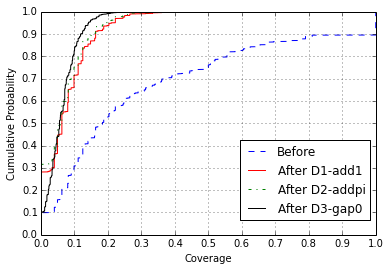
\includegraphics[width=0.5\textwidth]{fig/dist2}
\end{figure}



